\section{Referencia del Archivo /media/docs/progra/c++/compiladores1/proy2/godzilla/src/main.cpp}
\label{main_8cpp}\index{/media/docs/progra/c++/compiladores1/proy2/godzilla/src/main.cpp@{/media/docs/progra/c++/compiladores1/proy2/godzilla/src/main.cpp}}
Punto de entrada del programa. 

{\tt \#include $<$qapplication.h$>$}\par
{\tt \#include $<$string.h$>$}\par
{\tt \#include \char`\"{}parserheader.h\char`\"{}}\par
{\tt \#include \char`\"{}godzilla.h\char`\"{}}\par


Dependencia gr\'{a}fica adjunta para main.cpp:\begin{figure}[H]
\begin{center}
\leavevmode
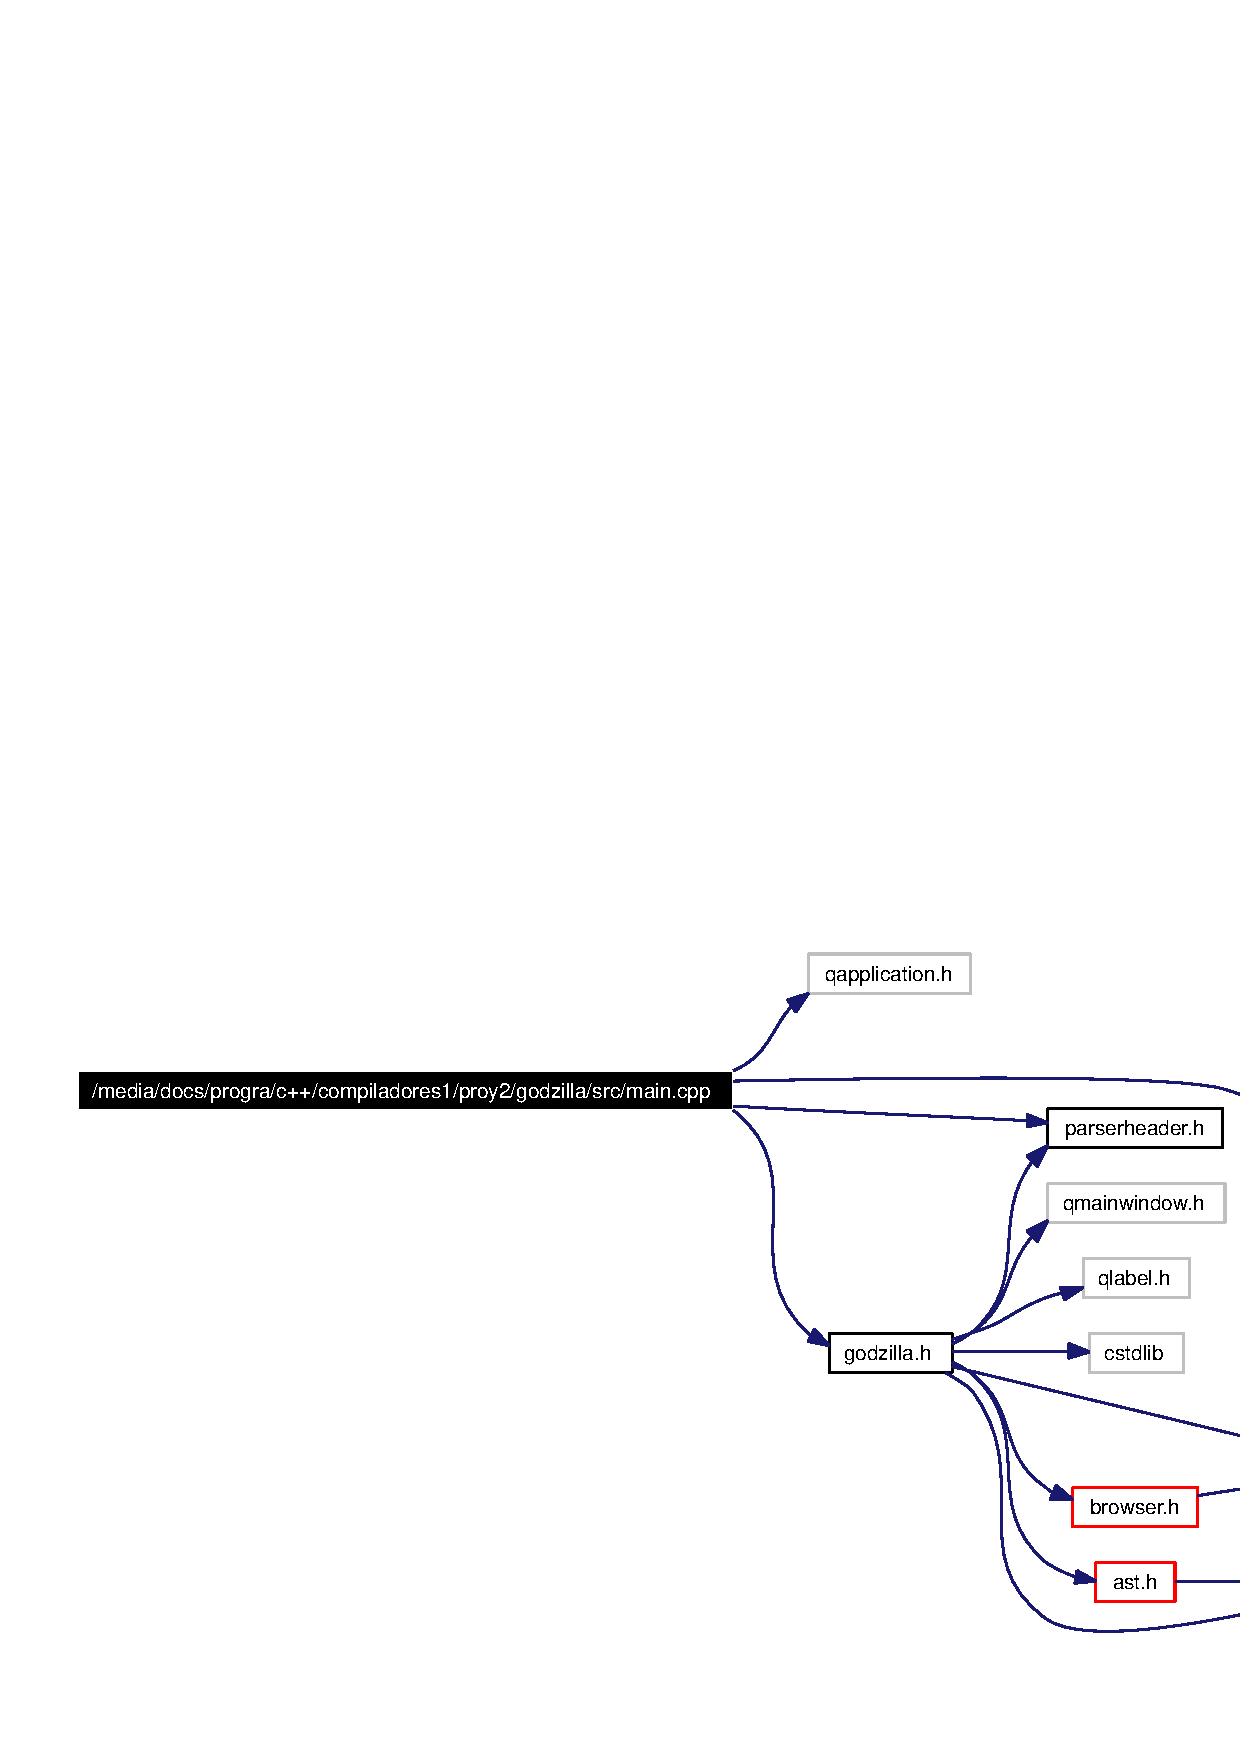
\includegraphics[width=396pt]{main_8cpp__incl}
\end{center}
\end{figure}
\subsection*{Funciones}
\begin{CompactItemize}
\item 
int {\bf main} (int argc, char $\ast$$\ast$argv)
\begin{CompactList}\small\item\em Crea objetos QApplication y {\bf God\-Zilla}{\rm (p.\,\pageref{classGodZilla})}, y los ejecuta para mostrar interfaz grafica. \item\end{CompactList}\end{CompactItemize}


\subsection{Descripci\'{o}n detallada}
Punto de entrada del programa. 



Definici\'{o}n en el archivo {\bf main.cpp}.

\subsection{Documentaci\'{o}n de las funciones}
\index{main.cpp@{main.cpp}!main@{main}}
\index{main@{main}!main.cpp@{main.cpp}}
\subsubsection{\setlength{\rightskip}{0pt plus 5cm}int main (int {\em argc}, char $\ast$$\ast$ {\em argv})}\label{main_8cpp_a0}


Crea objetos QApplication y {\bf God\-Zilla}{\rm (p.\,\pageref{classGodZilla})}, y los ejecuta para mostrar interfaz grafica. 



Definici\'{o}n en la l\'{\i}nea 16 del archivo main.cpp.

Hace referencia a generar\-Salida\-Error(), y inputparse().